%
% CMPT 473: Software Quality Assurance - A Course Overview
% Section: Graph Coverage
%
% Author: Jeffrey Leung
%

\section{Graph Coverage}
	\label{sec:graph-coverage}
\begin{easylist}

& \textbf{Control flow graph (CFG):} Graph where nodes represent code and edges represent paths taken
	&& Types of nodes: Entry, decision/branch, join, exit
	&& For a while loop, see figure~\ref{img:flow-diagram-while}
	&& For a for loop, see figure~\ref{img:flow-diagram-for}
	&& For a switch statement, see figure~\ref{img:flow-diagram-switch}
	&& For a short-circuited if statement, see figure~\ref{img:flow-diagram-if-shortcircuit}

\end{easylist}

\begin{figure}[!htb]
	\centering
	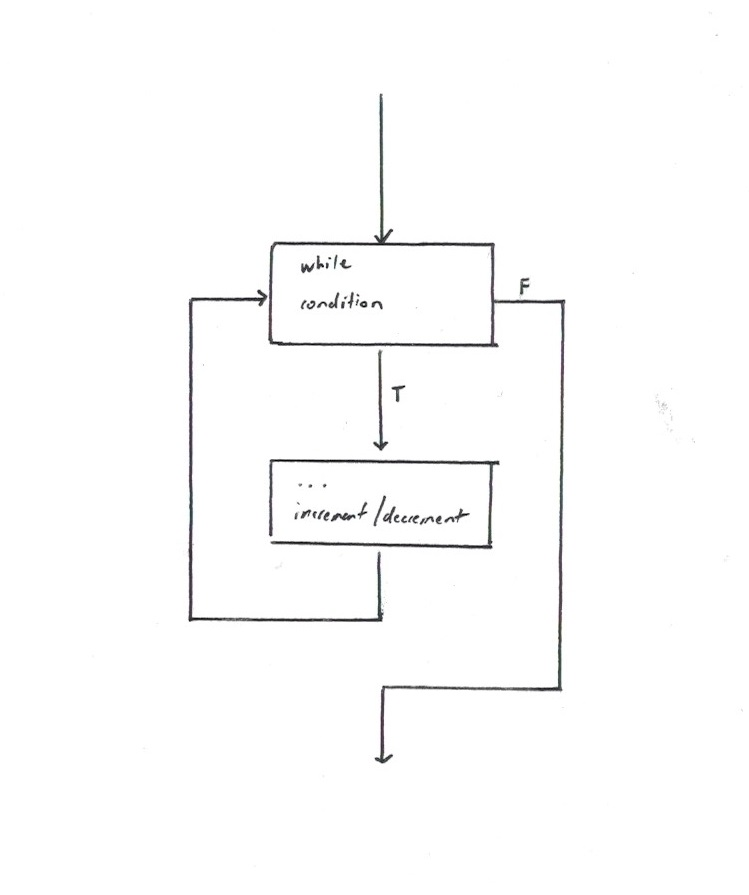
\includegraphics[width=.5\linewidth]{flow-diagram-while}
	\caption{Control Flow Graph of a while loop}
	\label{img:flow-diagram-while}
\end{figure}

\begin{figure}[!htb]
	\centering
	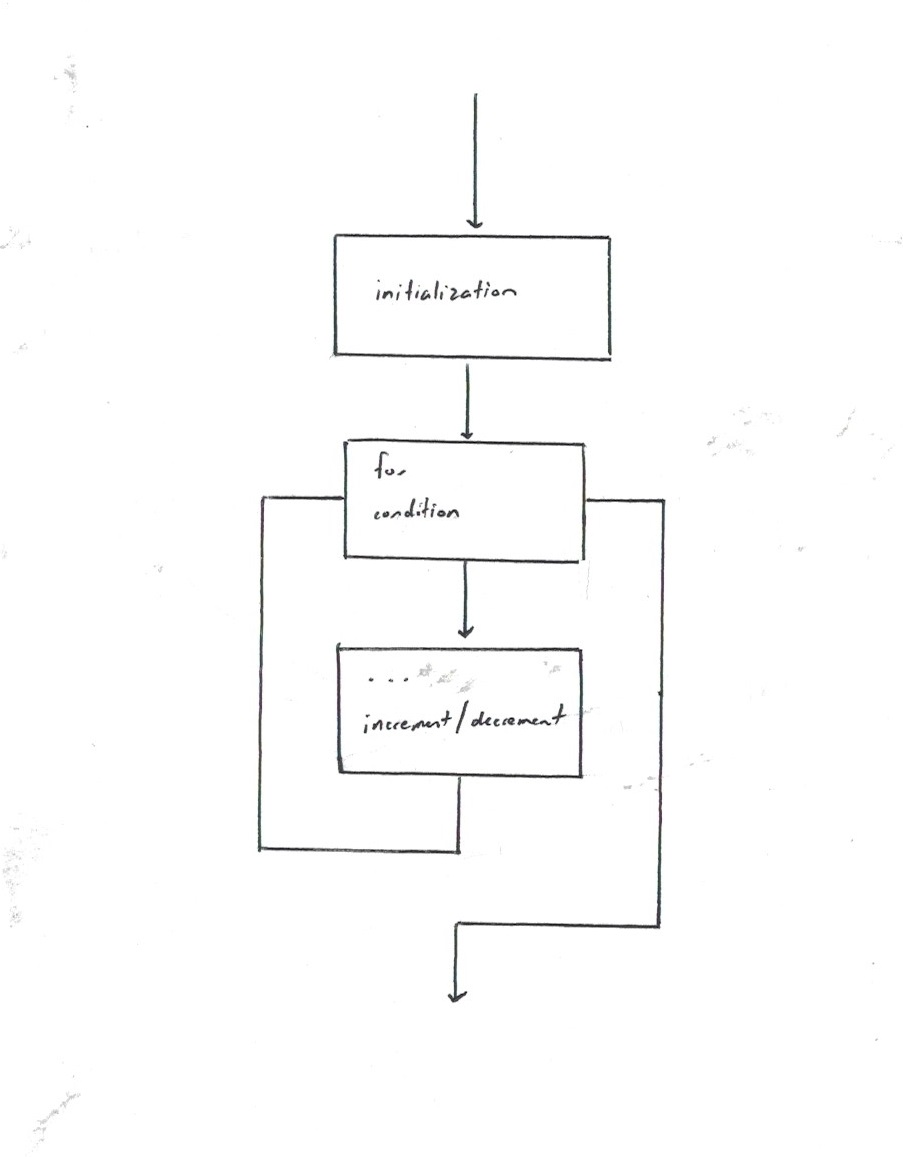
\includegraphics[width=.5\linewidth]{flow-diagram-for}
	\caption{Control Flow Graph of a for loop}
	\label{img:flow-diagram-for}
\end{figure}

\begin{figure}[!htb]
	\centering
	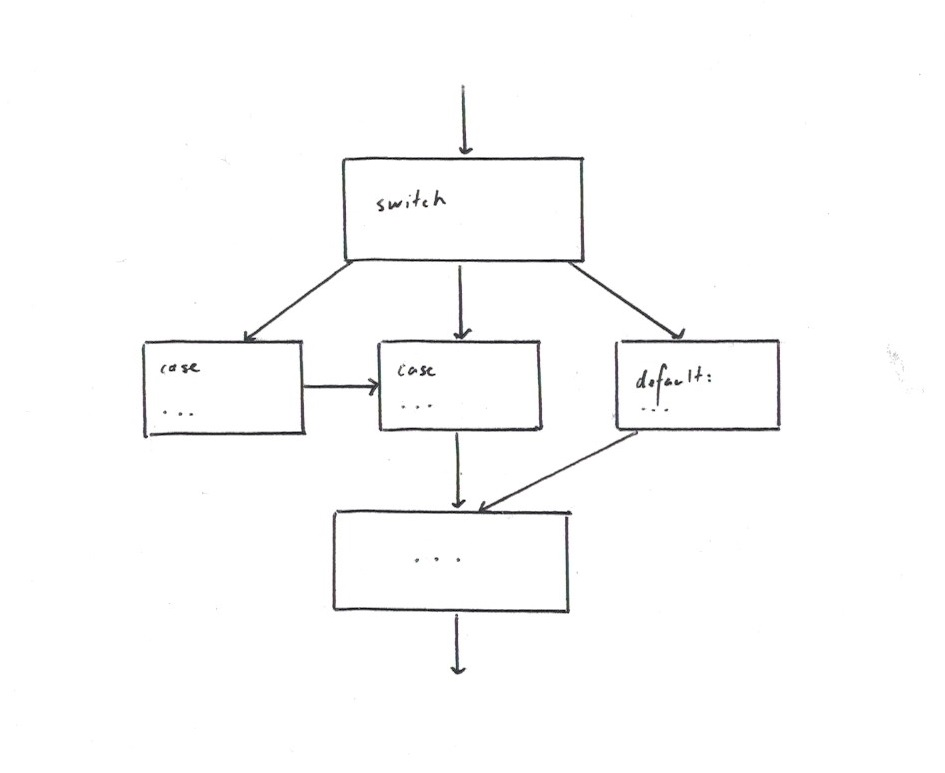
\includegraphics[width=.5\linewidth]{flow-diagram-switch}
	\caption{Control Flow Graph of a switch statement}
	\label{img:flow-diagram-switch}
\end{figure}

\begin{figure}[!htb]
	\centering
	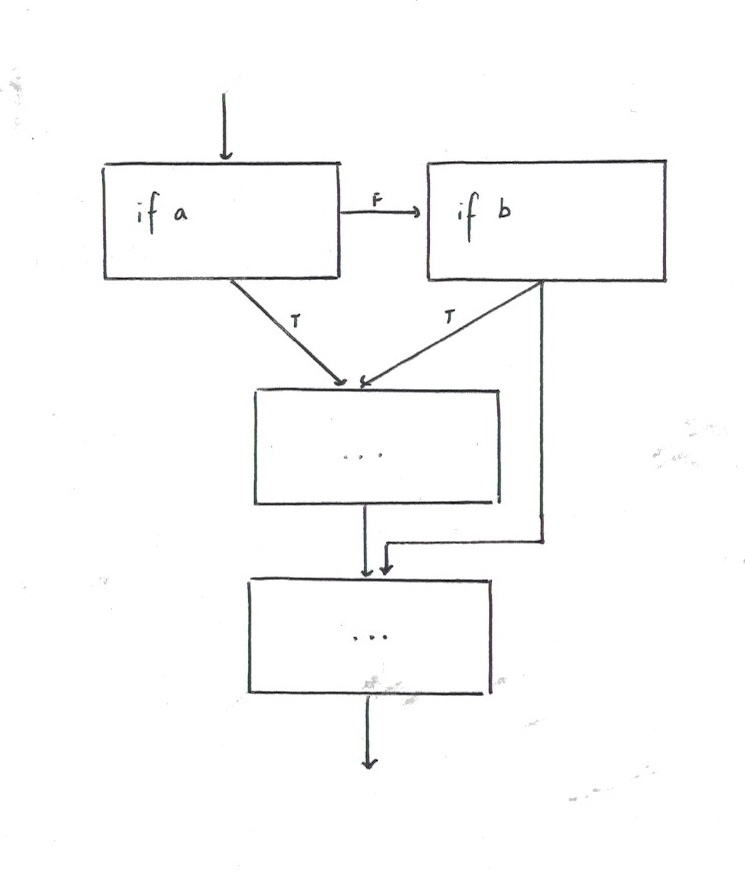
\includegraphics[width=.5\linewidth]{flow-diagram-if-shortcircuit}
	\caption{Control Flow Graph of a if statement short-circuited}
	\label{img:flow-diagram-if-shortcircuit}
\end{figure}

\begin{easylist}

& Edge coverage (i.e. all branches used) is a superset of node coverage

& \textbf{Complete path coverage:} Coverage of all possible paths through the graph
	&& Reason: Permutations/combinations of multiple possible paths can affect results
	&& Infeasible/intractible because it would entail combinatorial explosion and inability to efficiently test looping paths

& \textbf{Edge pair coverage:} Coverage which includes every path of length $<= 2$
& \textbf{Specified path coverage:} Coverage which tests $k$ paths for a given $k$

& \textbf{Reachability}: Property of a piece of code which may or may not be executable based on states
	&& \textbf{Syntactic reachability:} Analysis of reachability based on the structure of the code
	&& \textbf{Semantic reachability:} Analysis of reachability based on the meaning of the code (cannot be checked by an automated program)

& Testing loops is relevant when each iteration may affect the next
	&& \textbf{Simple path:} Acyclic path between nodes where no node appears more than once (except first/last)
	&& \textbf{Prime path:} Simple path which is not a subpath of any other simple path
		&&& I.e. A simple path which cannot be extended
		&&& E.g. Simple path which starts and ends at the same node
	&& \textbf{Tour:} Path which is a subpath of another
		&&& Mathematical definition: A path $p$ tours path $q$ if $q$ is a subpath of $p$
		&&& Tour with sidetrips: Tour where every edge of the superpath appears in the same order in the subpath
		&&& Tour with detours: Tour where every node of the superpath appears in the same order in the subpath

& \textbf{def-use pair:} Definition statement and the next relevant uses of the variable (before reassignment)
	&& Used to test along data flow
	&& Possible test approaches:
		&&& All defs coverage: Every def must be covered by at least one test of its uses
		&&& All uses coverage: Every use must be tested with least one definition
		&&& All def-use pairs coverage
		&&& All def-use paths coverage: All simple paths between def-use pairs are covered

& Path/branch coverage is insufficient due to scalability and complex conditions (e.g. non-short-circuiting) which do not have the notion of a path

\end{easylist}
\clearpage
